\chapter{Image Processing}
To locate objects in the manipulator workspace computer vision methods were used. The Creative Senz 3D depth sensing camera was used to gather depth and color data of the workspace. OpenCV was then used to locate objects in the read images. The depth data could than be used to actually calculate the xyz position of the found image location. This was the general method for locating objects in the manipulator's workspace.

\section{Creative Senz 3D}
The Creative Senz 3D camera produces three different outputs which is sends using USB; sound, depth data, and color images. Each of these is read in by the computer by connecting to the corresponding data streams. To make the camera Linux compatible the DepthSense Software Development Kit (SDK) was used. This software was designed for use with SoftKinetics's 3D cameras but currently works with the Creative Senz 3D. The SDK for the Creative camera was not used as it is a Window's only program. Linux compatability was important for future work to be able to put code to interface with the camera could by run on Odroid which runs a Linux operating system. 

\section{Depthsense SDK}
The DepthSense SDK libraries provide classes and functions for handling the camera data as well as sample code for reading in the data. The main function for gathering data initializes the color and depth nodes than waits for new data of each of those to be received. The nodes for color and depth can be configured to return the desired types of data. For example the different depth data types used in this project were the UV Map, depthMap, and VerticesFloatingPoint and the color data was colorMap. The colorMap data stores the Red Green Blue (RGB) values for each pixel in the color image. The depthMap and verticiesFloatingPoint stores the xyz coordinates of each depth point as calculated in the SDK. The UVMap data is used to convert between the depth image and color image. This is necessary because the depth image is not taken at the exact same place on the camera as the color image and the two images are not the same size. Therefore to find the depth at a color pixel coordinate or the color of a point on the depth map on a way to convert between them is necessary.

The v member of the uv map refers to the row, or height, of the color image and the v refers to the column or width of the color image. The conversion algorithm between color pixel coordinates to the uv coordinate is shown in algorithm \ref{alg:uv}.

\begin{algorithm}
	\begin{enumerate}
		\item Get UV map from DepthSenseSDK.
		\item colorImageRow = V member of UV * height of color image.
		\item colorImageColumn = U member of UV * width of color image.

	\end{enumerate}
\caption{Use UV map to convert from depth location to pixel coordinates.}
\label{alg:uv}
\end{algorithm}

Reading in the color image and depth image as well as converting between locations in the two is all that is necessary from the Depthsense SDK software. This code makes up the main part of the camera code. The main function calls the functions necessary to set up the nodes and then waits for data. Functions exist called OnNewDepthSample and OnNewColorSample which run every time new data of this type is received. It is in these functions where data was read into variables to be used for further analysis.

\section{Finding Depth Data at a Desired Location}
Once an object is located in the color image the xyz coordinates must be found. To do this the depth map is searched through and using the uv mapping technique discussed above the row and column of the color image is found for each depth point. If the row and column matches the xy position of the found object than that depth position in xyz coordinates, found by using the verticiesFloatingPoint depth data, is stored as the real world position of the image coordinates.

 For more consistent readings of depth an average of the points around the found object was used rather than just the center point. This is because there are some holes in the depth data, where it reads a default 0,0,0 coordinate. This happens most often when an object starts approaching the lower limit of range on the camera. The average was a way to avoid no data being returned in these situations. The area used was $\pm$ a third of the found objects bounding circle radius. This gives enough points to create a safe average while guaranteeing the area is always within the desired object regardless of size. 
 
 \begin{algorithm}
 	\begin{enumerate}
 		\item x,y = found pixel position in color image
 		\item radius = radius of objects bounding circle
 		\item boundaries = x,y$\pm$radius/3
 		\item for all depth data
 		\item use uv map to  find corresponding pixel location
 		\item if in boundaries save VerticesFloatingPoint to averaging point
 		\item take average of found XYZ coordinates 
 		\item filter found  coordinates
 	\end{enumerate}
 \caption{Find world coordinates of a pixel coordinate}
 \label{alg:cam}
 \end{algorithm}
 
 The found xyz position was also put through a low pass filter as the coordinates had a fair amount of noise. The filter used was a 3rd order Butterworth Filter whose equation is shown in equation \ref{eq:filter}. The derivation of this formula can be seen in Appendix 2. The algorithm for the camera coordinate to world coordinate position is shown in algorithm \ref{alg:cam}.

\begin{equation}
\label{eq:filter}
y = \frac{w_c^2x-2w_c^2xp+w_c^2xpp-yp(2w_c^2-\frac{8}{T^2})-4-ypp(w_c^2-\frac{2\sqrt{2}wc}{T}+\frac{4}{T^2})}{\frac{4}{T^2}+\frac{2\sqrt{2}w_c}{T}+w_c^2} 
\end{equation}
Where x is the current value, xp is the previous value, xpp is the previous previous value, yp is the previous filtered value, and ypp is the previous previous filtered value.

The final step in getting a usable xyz position is to convert from the camera coordinate frame to the base frame of the manipulator. The camera's coordinate frame is at the center point between the depth and color camera's and the manipulators coordinate frame is at the first joint of the manipulator. These frames are shown in Figure \ref{fig:mount}. The conversion between these frames is found by the equations in  \ref{eq:conv}.

\begin{subequations}
\label{eq:conv}
	\begin{align}
	x_{arm} = y_{cam} + a \qquad \\
	y_{arm} = x_{cam}  \qquad \\
	x_{arm} = z_{cam} - b 
	\end{align}
\end{subequations}

 Where distance a is the distance between $x_{arm}$ and $y_{cam}$ measured along the $z_{arm}$ axis and the distance b is the difference between $z_{arm}$ and $z_{cam}$ measured along the $x_{arm}$ axis. 

\begin{figure}
\centering
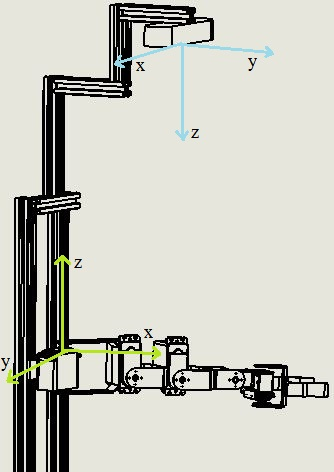
\includegraphics[width=0.3\textwidth]{armcoord}
\caption{Arm with Camera Mounted Above.}
\label{fig:mount}
\end{figure}

\subsection{Point Cloud Library}
The Point Cloud Library (PCL) is a library used for interpreting and using point clouds. Point clouds are a set of points in 3D space. These can refer to a pure depth image or also contain color information. PCL has a number of functions and examples for object recognition and tracking. It was possible to import the depth data from the camera into point cloud form and view using PCL's viewing functions. The PCL functions for object recognition did not turn out to be reliable for this project. The alternative looked at was Open Source Computer Vision (OpenCV) which more reliably found objects with the camera data. 

\subsection{Open CV}
OpenCV is another library with image processing functions which works across different computer languages and operating systems. The DepthSense SDK was written in C++ so the C++ version of OpenCV functions were utilized in this project. OpenCV has a number of different functions such as color detection, finding contours, shape fitting, and image filtering. Many of these functions were used for object detection in this project.

\subsection{First Version}
The first version of object detection was written based on color. First the color image was save as a Mat, or matrix type, which is how OpenCV saves images. The image was then converted from an RGB to HSV (Hue, Saturation, and Value). HSV has an advantage over RGB for color detection as it is easy to cover a range of saturations for a particular color, or hue, by only changing the saturation value rather than recalculating the RGB values for a slight change in saturation. The HSV range of the color was saved and compared to the pixels in the color image. A matrix of the same size was saved with a one if the pixel was in range and a zero if it was not. The result is a binary image, which is viewed as a black and white image, white for a value of one and black for a value of zero. This image was then put through filtering functions to remove holes and small objects caused by noise in the color image and the result is the object found in the image of that color.

The contours of the binary image were then found. Contours are the enclosing shapes found around the edges of an image. Assuming only one object of the desired color is in the image all found contours were merged. The OpenCV function to find the minimum enclosing circle around a contour was used to return the center point and radius of the found object. 

\begin{figure}
    \centering
    \begin{subfigure}[b]{0.3\textwidth}
    	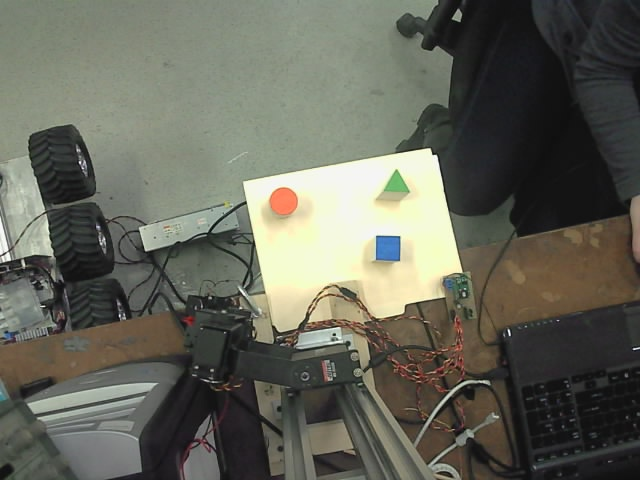
\includegraphics[width=\textwidth]{origional}
    	\caption{Original color image. }
    	\label{fig:image1}
   	 \end{subfigure}
   	 \quad
    \begin{subfigure}[b]{0.3\textwidth}
		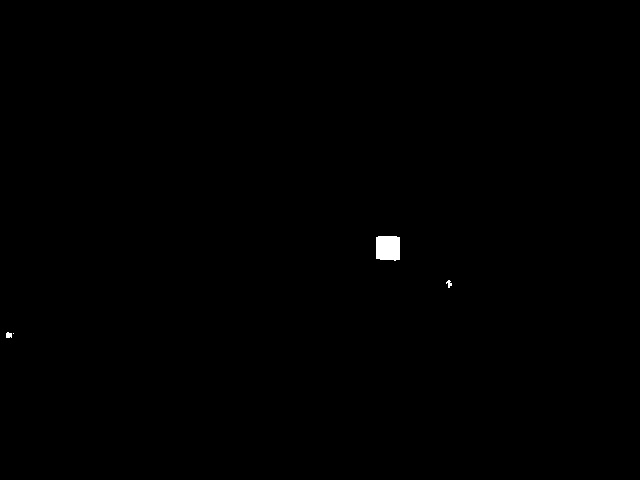
\includegraphics[width=\textwidth]{threshold}
		\caption{Binary image of found blue color before filtering. }
		\label{fig:image2}
    \end{subfigure}
    \quad %add desired spacing between images, e. g. ~, \quad, \qquad, \hfill etc.
    \begin{subfigure}[b]{0.3\textwidth}
        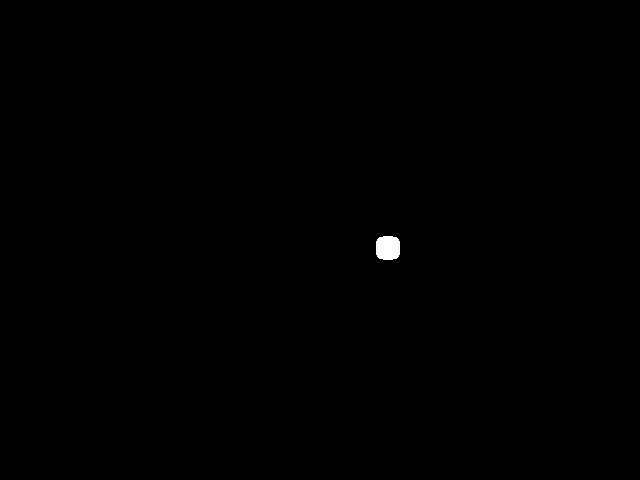
\includegraphics[width=\textwidth]{filteredthreshold}
        \caption{Binary image of found blue color after filtering.. }
        \label{fig:image3}
    \end{subfigure}
    \quad
    \begin{subfigure}[b]{0.3\textwidth}
       	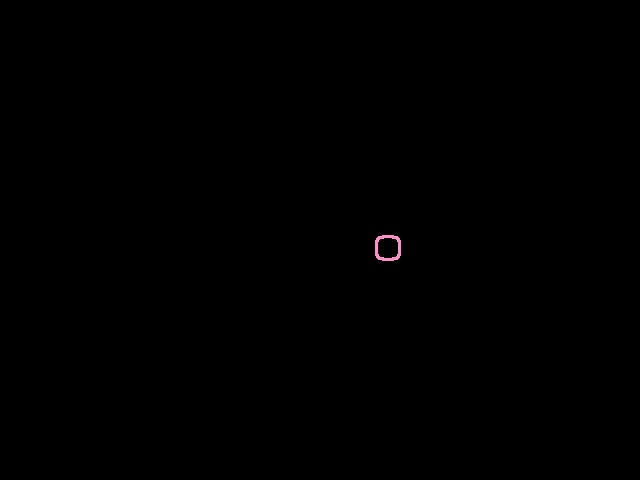
\includegraphics[width=\textwidth]{contourimage}
       	\caption{Found contours of blue object. }
       	\label{fig:image4}
   \end{subfigure}
    \quad
    \begin{subfigure}[b]{0.3\textwidth}
        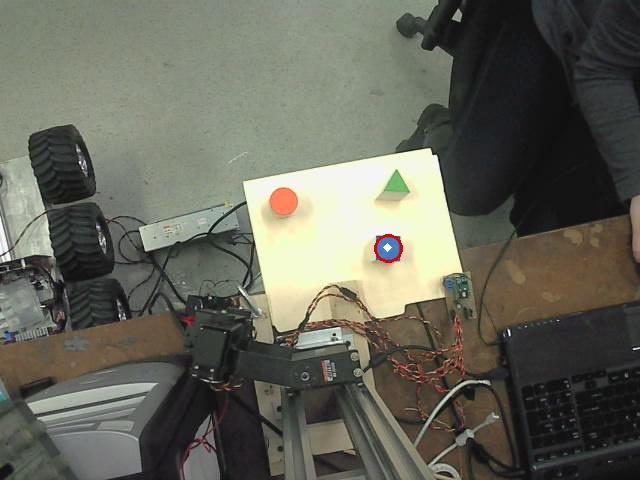
\includegraphics[width=\textwidth]{final}
        \caption{Minimum enclosing circle drawn around found object in original image. }
        \label{fig:image5}
    \end{subfigure}
    \quad
      %(or a blank line to force the subfigure onto a new line)
 	\caption{Locating a blue object in camera image. }
 	\label{fig:imag}
\end{figure}


The code for this object location program is shown in Appendix C. While this code worked consistently it did have limitations. As stated above it relies on the assumption that only one object of the desired color is present in the camera image. If there is more than one the center point returned will be somewhere in between with a radius big enough to contain all objects of that color. The program also find the minimum enclosing circle of the object regardless of its shape. This means there is no way to determine the difference between a circle, square, or any other shape in this code. It was therefore necessary to create a more well rounded algorithm for object detection.

An example of this can be seen in the images of Figure\ref{fig:imag}. To track an object of the color blue the HSV values were found to be: H = 100 - 130, S = 100-255, V = 49-255. The original image is shown in Figure \ref{fig:image1}. The thresholded image before filtering, after finding blue, is shown in Figure \ref{fig:image2} and after filtering in Figure \ref{fig:image3}. The found contours of the image are shown in Figure \ref{fig:image4} and finally the minimum enclosing circle drawn onto the image along with the found center point is shown in Figure \ref{fig:image5}. This program ran fast enough to track an object in real time and calculate 3D coordinates. Viewing the results on screen has no noticeable delay.


\subsection{Second Version}
To fix the limitations seen from the first version of the code a new version was written based on basic shape detection. The goal is to find basic shapes, such as circles, triangles, and squares from a color image. 

Shape detection started out similar to the color tracking code by creating a binary image for selected colors. For testing purposes the color selection was set to select all but the background colors. Using a binary image is much more reliable for the contour and shape detection functions in OpenCV which is why there is still a color based part to this code. This image was left unfiltered as the filtering process used in the color method rounds out the shapes too much for any kind of detection to work. Since the objects used in this project are so small in camera frame even a little bit of smoothing cuts off the corners needed for shape detection. Therefore the unfiltered image was put in the find contours function.

To then ignore all the smaller shapes only the convex contours with a larger area were looked at. Both area and convexity of a contour can be checked with OpenCV functions. For each contour meeting this criteria the approximate polygon  function was used which returns a set of vertices's for the contour. To detect the shapes the number of vertices's was used. The three shapes recognized for this program were triangle, square, and circle. The shapes were determined by the appropriate number of vertices's, for a square four and for a triangle three. The circle was marked as found for any contours with five or more vertices's. Normally this would be assumed to be a larger number but since the objects were small the approximate polygon function often found the circle to have only five vertices's. To restrict the conditions of shape further the angles between the vertices's can also be calculated. So for a square all the angles should be approximately 90 degrees, for a triangle the angles should sum to around 180 degrees, and so on. For this situation the shapes were located more easily without adding these extra conditions. There was too much noise present in the image and adding this extra angle constraint resulted in no shapes being found most of the time. Since just the vertices's condition worked much better this was the only criteria used for shape matching.

 Once found the program drew a line between all vertices's on the image and labeled it with the shape it was determined to be. An image of this working is shown in Figure \ref{fig:shapes}.

\begin{figure}
\centering
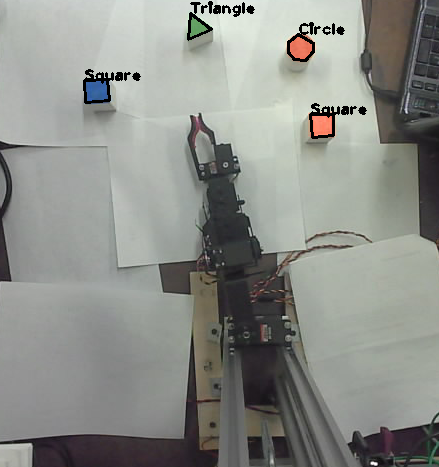
\includegraphics[width=0.5\textwidth]{shapesall.png}
\caption{Shapes located in image, labeled by program.}
\label{fig:shapes}
\end{figure}

This method often read incorrect shapes without a clean workspace. It always found the objects but did not estimate them to have the correct number of vertices. When putting the objects onto a white background enough noise was eliminated to make this method much more reliable.

To find the coordinates of the center of the shape a geometric method can be used based on the shape found. For a square the center is found as halfway from the distance of two adjacent sides. A triangle center is found as halfway between the center of one side and the opposite point. The simplest method for finding the center of the circle was to use the minimum bounding circle function on the circle contour. 

To locate all of the objects in the workspace for this experiment a combination of color and shape locating was used. Given an object for input first the color of the object is found and a binary image created for just that color. That image is then searched for the corresponding shape of the obstacle and the center point is returned. With this modification more than one object of the same color can be present in the image and an accurate result produced. 

 While this code was tested with the same workspace as used for the manipulator, the first version of the code was used for this project. The first version had less room for error and was simpler to implement. This version does provide a future more robust alternative. The code for both versions of the image code can be found in Appendix A.
